%\addcontentsline{toc}{chapter}{Development Process}
\chapter{Experiment Methods}

%This section should discuss the overall hypothesis being tested and justify the approach selected in the context of the research area.  Describe the experiment design that has been selected and how measurements and comparisons of results are to be made.

%You should concentrate on the more important aspects of the method. Present an overview before going into detail. As well as describing the methods adopted, discuss other approaches that were considered. You might also discuss areas that you had to revise after some investigation.

%You should also identify any support tools that you used. You should discuss your choice of implementation tools or simulation tools. For any code that you have written, you can talk about languages and related tools. For any simulation and analysis tools, identify the tools and how they are used on the project.

%If your project includes some engineering (hardware, software, firmware, or a mixture) to support the experiments, include details in your report about your design and implementation. You should discuss with your supervisor whether it is better to include a different top-level section to describe any engineering work.

\section{Overview}

In order to test the main hypothesis of \say{Does the use of fuzzy entropy alignment metrics improve the alignment of mammograms?} an application was needed to portray the visual output. It would be built to take a set of input images, allow the user to select the alignment metric plus select how many iterations they would like completed and output the final congealed image. Details of the decreasing entropy would be a key output, along with the average image after each iteration completed, for a full picture of improvements.

However, the decisions about how to implement membership, which fuzzy entropy algorithms to use and which image alignment techniques remain.

\subsection{Pixel Membership}
\label{sssec:member}

From the analysis of the planned fuzzy entropy algorithms, one major task to be undertaken would be to calculate the membership of each pixel. Membership stems from Fuzzy set theory, as outlined in Subsection \ref{ssec:fuzzy-entropy}.

There are two common methods to modelling degrees of membership. The first is to manually define the category boundaries, so in the case of trapezium functions, the two bases and the two shoulders. The other solution would be to iterate over the image values have and to computationally build an even distribution throughout the membership functions, as in Strange and Mac Parthal\'ain \cite{Mac_Parthalain_Strange_2013}. Whilst this is the preferred method for being dynamical in its calculations, it is also more computationally expensive as pre-processing of the image would have to be completed before the \Gls{Congealing} algorithm could be run.

Taking the computational-expense into account, for grey-level pixel values, ranging from 0 (black) to 255 (white), two or three trapezium functions would be sufficient, therefore modeling `Low', `Medium' and `High' grey-level values. The bases and shoulders would be statically defined, as in Figure \ref{fig:3-trapeziums} and Table \ref{table:values}. For Non-Probabilistic entropy the highest membership for each pixel from each of the three trapezia would be taken as the membership degree. Hybrid entropy would take a slightly different approach, which will be covered later.

\begin{figure}[H]
  \center
  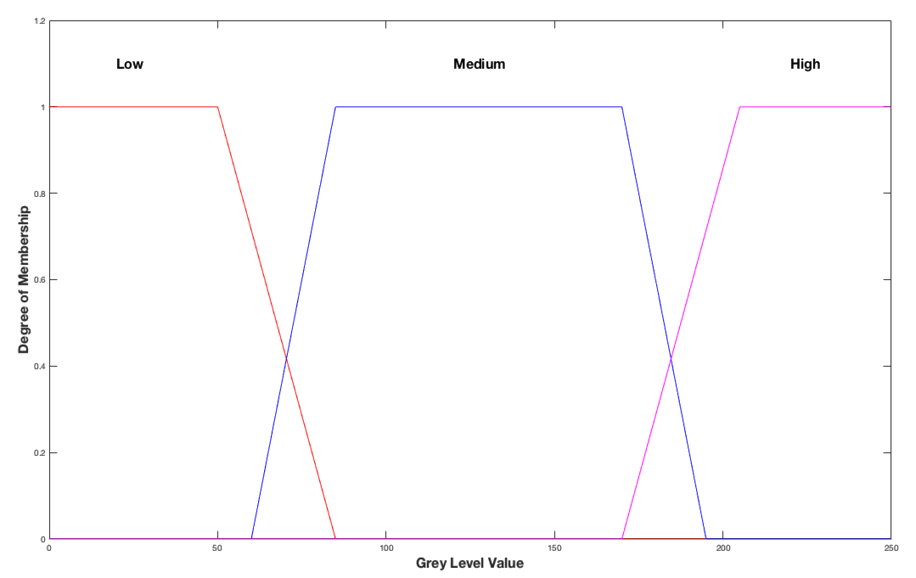
\includegraphics[scale=0.4]{Chapter2/hybrid-img/3_traps.png}
  \caption{3 trapezium-shaped membership sets}
  \label{fig:3-trapeziums}
\end{figure}

\begin{table}
  \center
  \begin{tabular}{ |l|l|l|l|l|l|l|l|l| }
    \hline
    \multicolumn{4}{|c|}{Low} & \multicolumn{5}{|c|}{} \\
    \hline
    \multicolumn{2}{|c|}{} & \multicolumn{5}{|c|}{Medium} & \multicolumn{2}{|c|}{}  \\
    \hline
    \multicolumn{5}{|c|}{} & \multicolumn{4}{|c|}{High} \\
    \hline
    0 & 50 & 60 & 70.4 & 85 & 170 & 195 & 205 & 255 \\
    \hline
    \cellcolor[gray]{0} & \cellcolor[gray]{0.19} & \cellcolor[gray]{0.24} & \cellcolor[gray]{0.28} & \cellcolor[gray]{0.33} & \cellcolor[gray]{0.66} & \cellcolor[gray]{0.76} & \cellcolor[gray]{0.8} & \cellcolor[gray]{1} \\ \hline
  \end{tabular}
\caption{Intepretation of the fuzzy sets across greyscale values}
\label{table:values}
\end{table}

\subsection{Fuzzy entropy choices}

\textbf{Chosen algorithms:}
\begin{itemize}
  \item Non-Probabilistic Entropy
  \item Hybrid Entropy
\end{itemize}

Given the simplistic nature of Non-Probabilistic entropy, this was one of the chosen fuzzy entropy algorithms to be implemented in the project.

Hybrid entropy was chosen for implementation in this project due to its hybrid nature (implementing both Probabilistic and Possibilistic uncertainty) and for its simplification nature - in the absence of fuzziness, then $E_0$ and $E_1$ reduce to $p_0$ and $p_1$ respectively, therefore classical Shannon entropy. This is especially useful in image processing, and other such areas which deal with a lot of noise.

Additionally, Shannon Entropy has already been implemented by Learned-Miller`s Congealing algorithm \cite{joint-alignment}, so this offers a non-fuzzy alternative to image alignment.

\textbf{Discarded algorithms:}
\begin{itemize}
  \item Fuzzy Shannon Entropy
  \item Higher Order Entropy
\end{itemize}

The initial plan was to implement the Fuzzy Shannon entropy algorithm in the project - however after further investigation which revealed that the algorithm does not model Probabilistic uncertainty - it was decided that it was to be excluded.

This project does not implement Higher Order Fuzzy Entropy due to the computational-overhead needed to run - especially on images with as much detail as a mammogram.


\subsection{Image Alignment choice}

\textbf{Image Alignment choice:}
\begin{itemize}
    \item \Gls{Congealing} algorithm
\end{itemize}

As this project will be working with mammograms, something with little variation nor inconsistency, \Gls{Congealing} is the perfect, light-weight image alignment algorithm to build upon, especially as the demonstration code available for research has a Shannon entropy implementation already developed.

\textbf{Discarded Image Alignment choice:}
\begin{itemize}
    \item Least squares \gls{Congealing}
    \item Joint Alignment of Complex Images
\end{itemize}

Least squares \gls{Congealing} algorithm was disregarded for this project due to the preference to focus upon entropy-based alignment algorithms and the computational costs that the authors themselves regard to be a drawback of their algorithm.

The Complex Images implementation of \Gls{Congealing} was quickly identified as overly complex for this project. The original \Gls{Congealing} algorithm was more appropriate for grey-scale mammograms, with a consistent canonical pose.

\section{Implementation tools}

This section will going into detail about the tools and programming language used to implement the application built to support the hypotheses.

\subsection{Tool \& Programming Language: MATLAB}
\label{ssec:matlab}

MATLAB \cite{MATLAB:2016} was chosen as the main implementation tool and programming language for the project as it is specifically designed to aid in scientific research. Furthermore, MATLAB was the ideal choice as the original \Gls{Congealing} algorithm was implemented in MATLAB. Other alternative languages, as outlined below, were ruled out:

\begin{itemize}
  \item Java: after contacting Learned-Miller directly, it was concluded that there was no \Gls{Congealing} algorithm demo code programmed in Java. The author did not want to further increase the workload to create a Java implementation as this could put the project at risk of non-completion.
  \item C++: the author decided not to persue using a C++ implementation of the \Gls{Congealing} algorithm, as in the public Git repository by `Debonet' \cite{cpp_congealing}, due to lack of experience in the language.
\end{itemize}

MATLAB offers a lot of built-in packages designed to alleviate the more mundane implementation tasks, such as reading in images (function \texttt{imread}) and applying functions to every item in a matrix (function \texttt{bsxfun}). This also leads to quicker run-times as MATLAB relies heavily on vectorisation of code (as outlined later in the document - Section \ref{sec:tech-diff}), which reduces the time spent running \texttt{for} loops.

However, to use MATLAB as a student, a license must be purchased. This costs \pounds29 + VAT as a stand-alone product, with additional Toolboxes costing an extra \pounds16 each. The open-source alternative Octave \cite{octave} was considered for a while, however due to original code having been developed in MATLAB, converting it over to Octave may have raised technical issues before the project has even begun.

\subsection{Tool: Version Control}

Version control is an important tool in modern day software creation. It records changes to files (such as code or written documents), and allows the user to update versions, or rollback to a previous version. In teams this is vital due to developers often working on the same, or similar, pieces of code simultaneously.

The tools utilised for version control in this project were Git \cite{2014gits}, Github online \cite{github} and Github desktop tool \cite{github_desktop}.

Git \cite{2014gits} is one of the most popular in terms of \acrfull{SCM} tools. It is a command-line tool which allows you to work on sections of code completely independent of each other and later merge them back into one complete article. Due to being written in C, Git is extremely quick compared to its rivals, being up to 325 times faster than \acrfull{SVN} \cite{About_Git}.

Github \cite{github} - \url{github.com} - is an online hosting service for Git repositories. It allows the user to clearly see all the files in the repository, make minor changes via an online editor, and to easily track features such as issues and feature requests. By offering both public and private repositories Github allows developers to work on new, incomplete projects that only they or their team can see, or to open-source their completed software and make it freely available to the world.

Github also allows visualisations of the commit history to the repository, as demonstrated in Figure \ref{fig:git-graph}.

\begin{figure}[H]
  \centering
  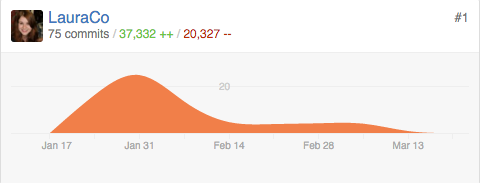
\includegraphics[width=0.6\textwidth]{Chapter2/tools/git_graph.png}
  \caption{Graph outlining git commit history in one branch during the project.}
  \label{fig:git-graph}
\end{figure}

Github desktop \cite{github_desktop} is a simple tool which leverages the power of both Git and Github. It allows the user to run commands usually executed via the command line in a \acrshort{GUI} and provides a graphical representation of the repository being worked in. This reduces the complexity of using branches, as the user can simply compare their current branch against others, and pull, push, merge and create pull requests as desired. Due to it being created by Github, instead of a third party, this ensures that Git is always up to date, and it seemlessly links in with the online project repository.

In order to sustain a solid Git flow each new feature, such as Hybrid entropy implementation or \acrshort{GUI} implementation, was developed in its own branch. Each new feature was branched off of the  main development branch, so the content was always up to date. Once a feature had been completed, changes would be pushed back up to the development branch, ready for the next feature to leverage the functionality.

\section{Dataset}

Whilst mammographic images are the dataset of choice, this project could be applied to any grey-scale image set, such as other medical imagery. The choice to use mammographic images was a personal one due to family history and an interest in aiding medicine via computer science techniques.

There exists several open mammogram datasets, so there was no issues in obtaining data without ethical concerns. The ethics form completed for the University can be found in Appendix \ref{appendix:ethics}. This section will outline the main open datasets considered for this project.

\subsection{Mammographic Image Analysis Society (MIAS) database}

The chosen dataset is a version of the \acrfull{MIAS}'s database, as it is commonly used within the research field and compiled for the sole purpose of trying to better understand mammograms. The original \acrshort{MIAS} database has been refined to create the Mini-\acrshort{MIAS} database which contains the same data, however with a size of 1024x1024 pixels. This size is preferable over the original \acrshort{MIAS} data, as it is a lot quicker to process.

Examples of Mini-\acrshort{MIAS} scans can be found throughout the document, however for reference, an example can be seen in Figure \ref{fig:mini-mias}

\begin{figure}[H]
  \centering
  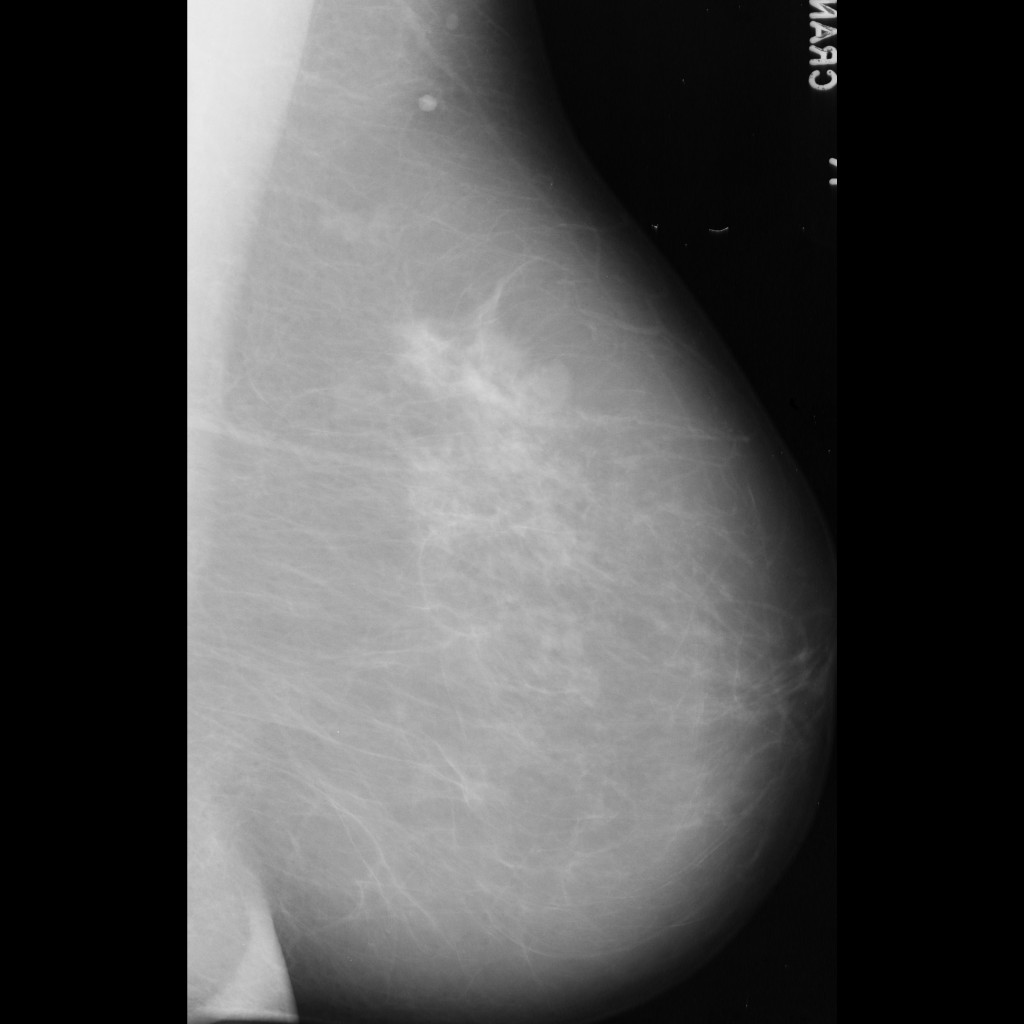
\includegraphics[width=0.4\textwidth]{Chapter2/tools/mias.jpg}
  \caption{Example Mini-MIAS scan, scaled down for inclusion in document.}
  \label{fig:mini-mias}
\end{figure}

\subsection{Other datasets}

\noindent \textbf{Digital Database for Screening Mammography (DDSM)}

The \acrshort{DDSM} database was created after a collobration between Massachusetts General Hospital, Sandia National Laboratories and the University of South Florida Computer Science and Engineering Department and contains around 2,500 scans \cite{Heath_Bowyer_Kopans_Moore_Kegelmeyer_Processing} \cite{Heath_Bowyer_Kopans_Kegelmeyer_Moore_Chang_MunishKumaran_1998}.
However, like the original \acrshort{MIAS} database, the images available via the DDSM are extremely large, and therefore unsuitable for this project due to the time it would take to process.

\noindent \textbf{Mammographic Mass Data Set}

As the name suggests, this dataset contains 961 instances of scans containing masses - both benign and malignant \cite{Elter_Schulz-Wendtland_Wittenberg_2007}. This project aims to work with solely healthy tissue, therefore this dataset is not beneficial.
